\section*{Appendix: Figure Captions}

\begin{figure}[h]
\centering
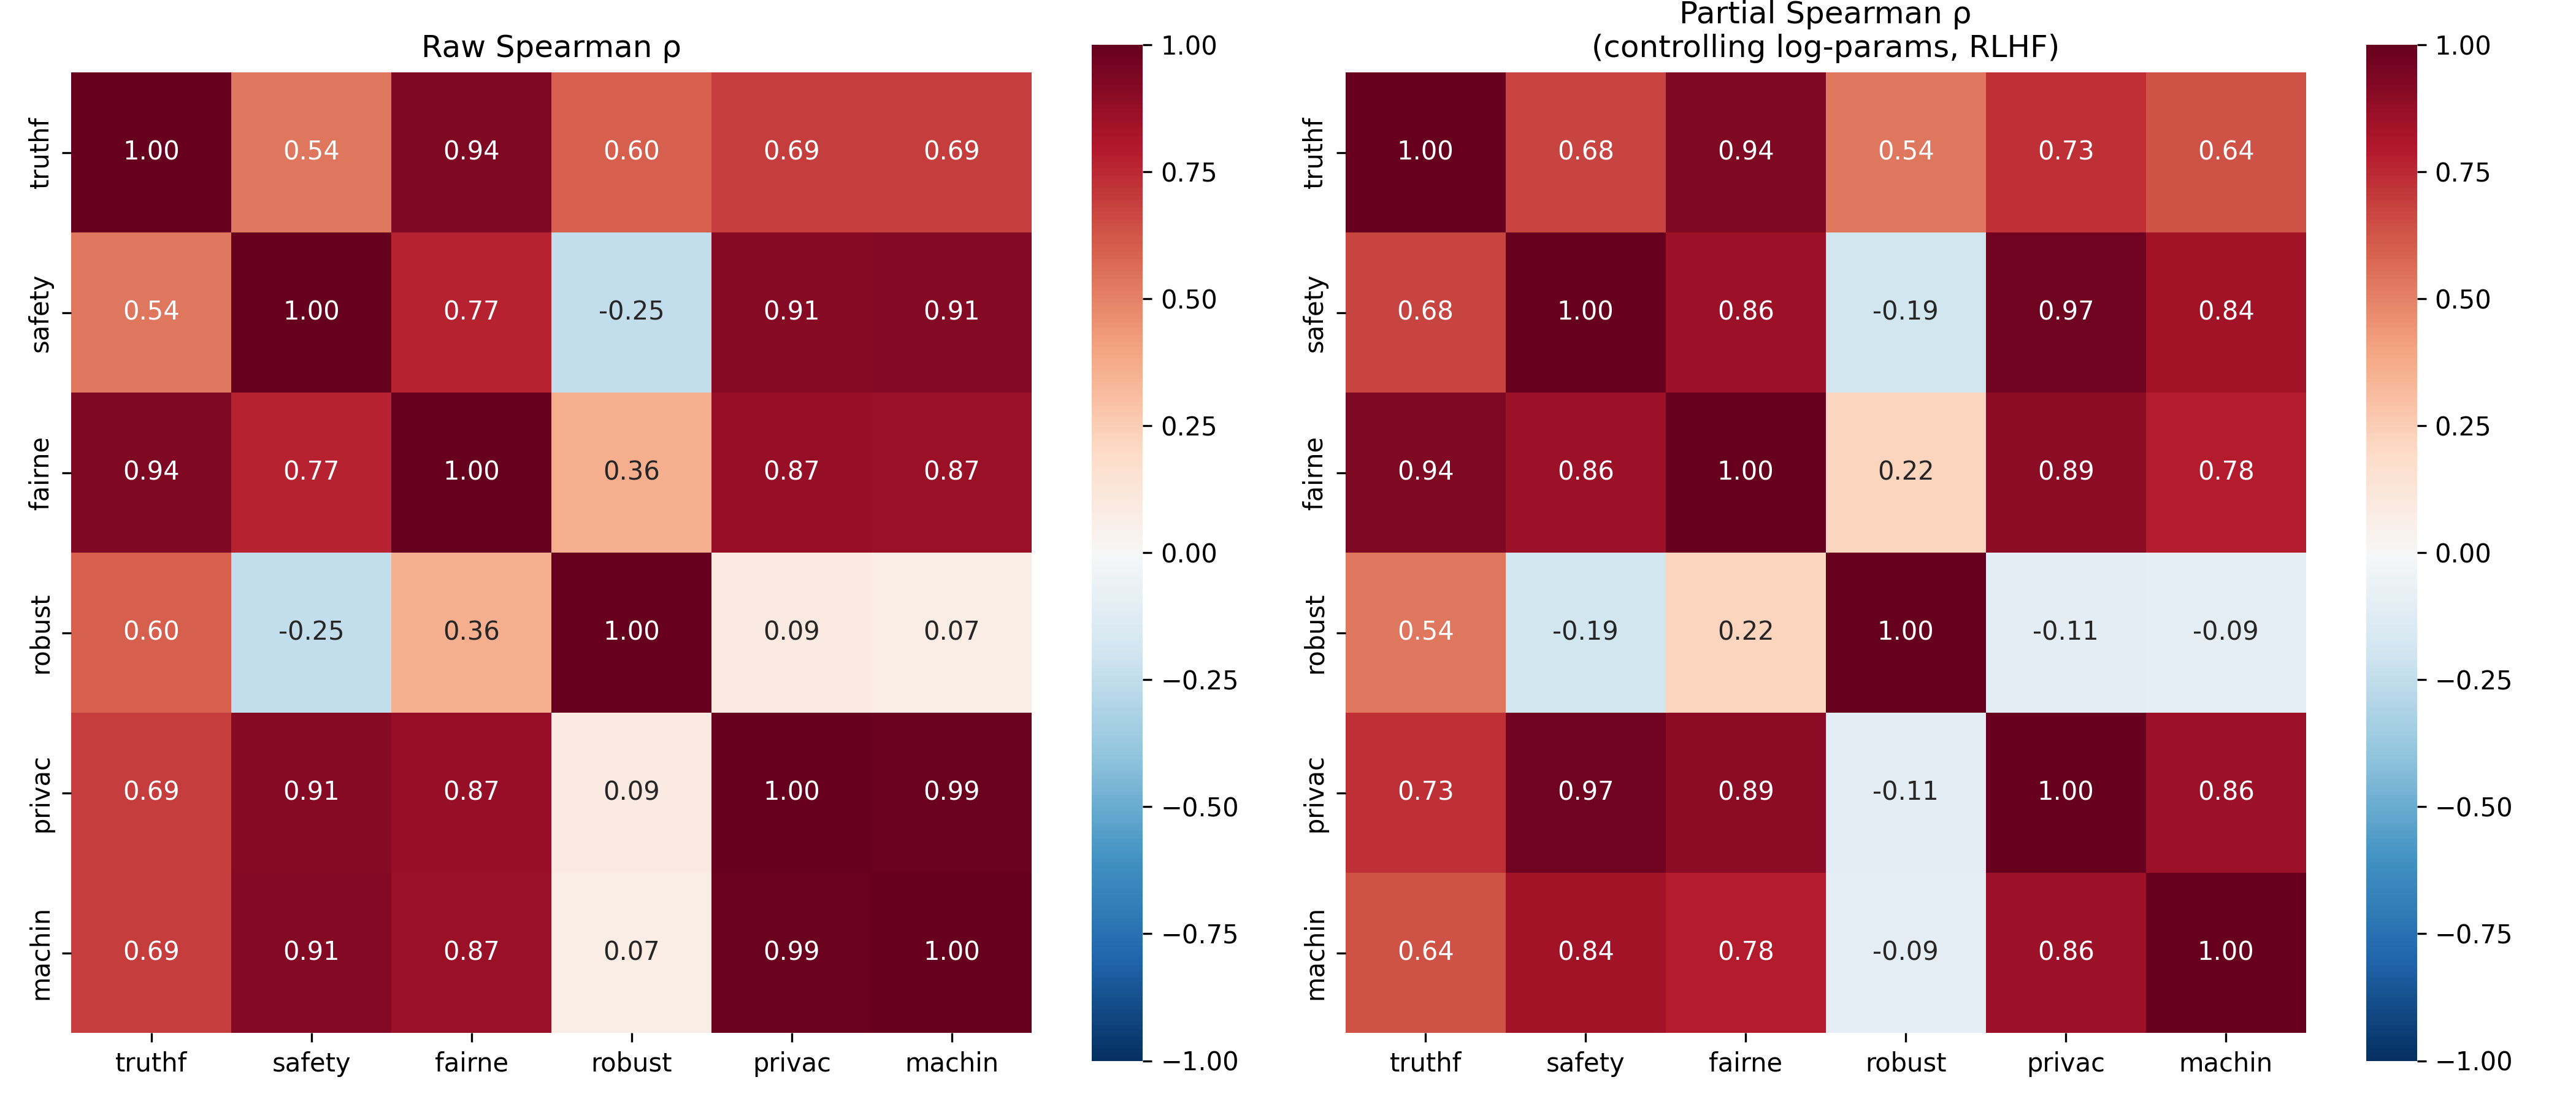
\includegraphics[width=\linewidth]{figures/02_heatmaps.png}
\caption{Side-by-side comparison of raw Spearman (left) and partial Spearman (right) $6 \times 6$ correlation heatmaps. Controlling for model scale and RLHF status reveals the underlying trustworthiness geometry.}
\label{fig:heatmaps}
\end{figure}

\begin{figure}[h]
\centering
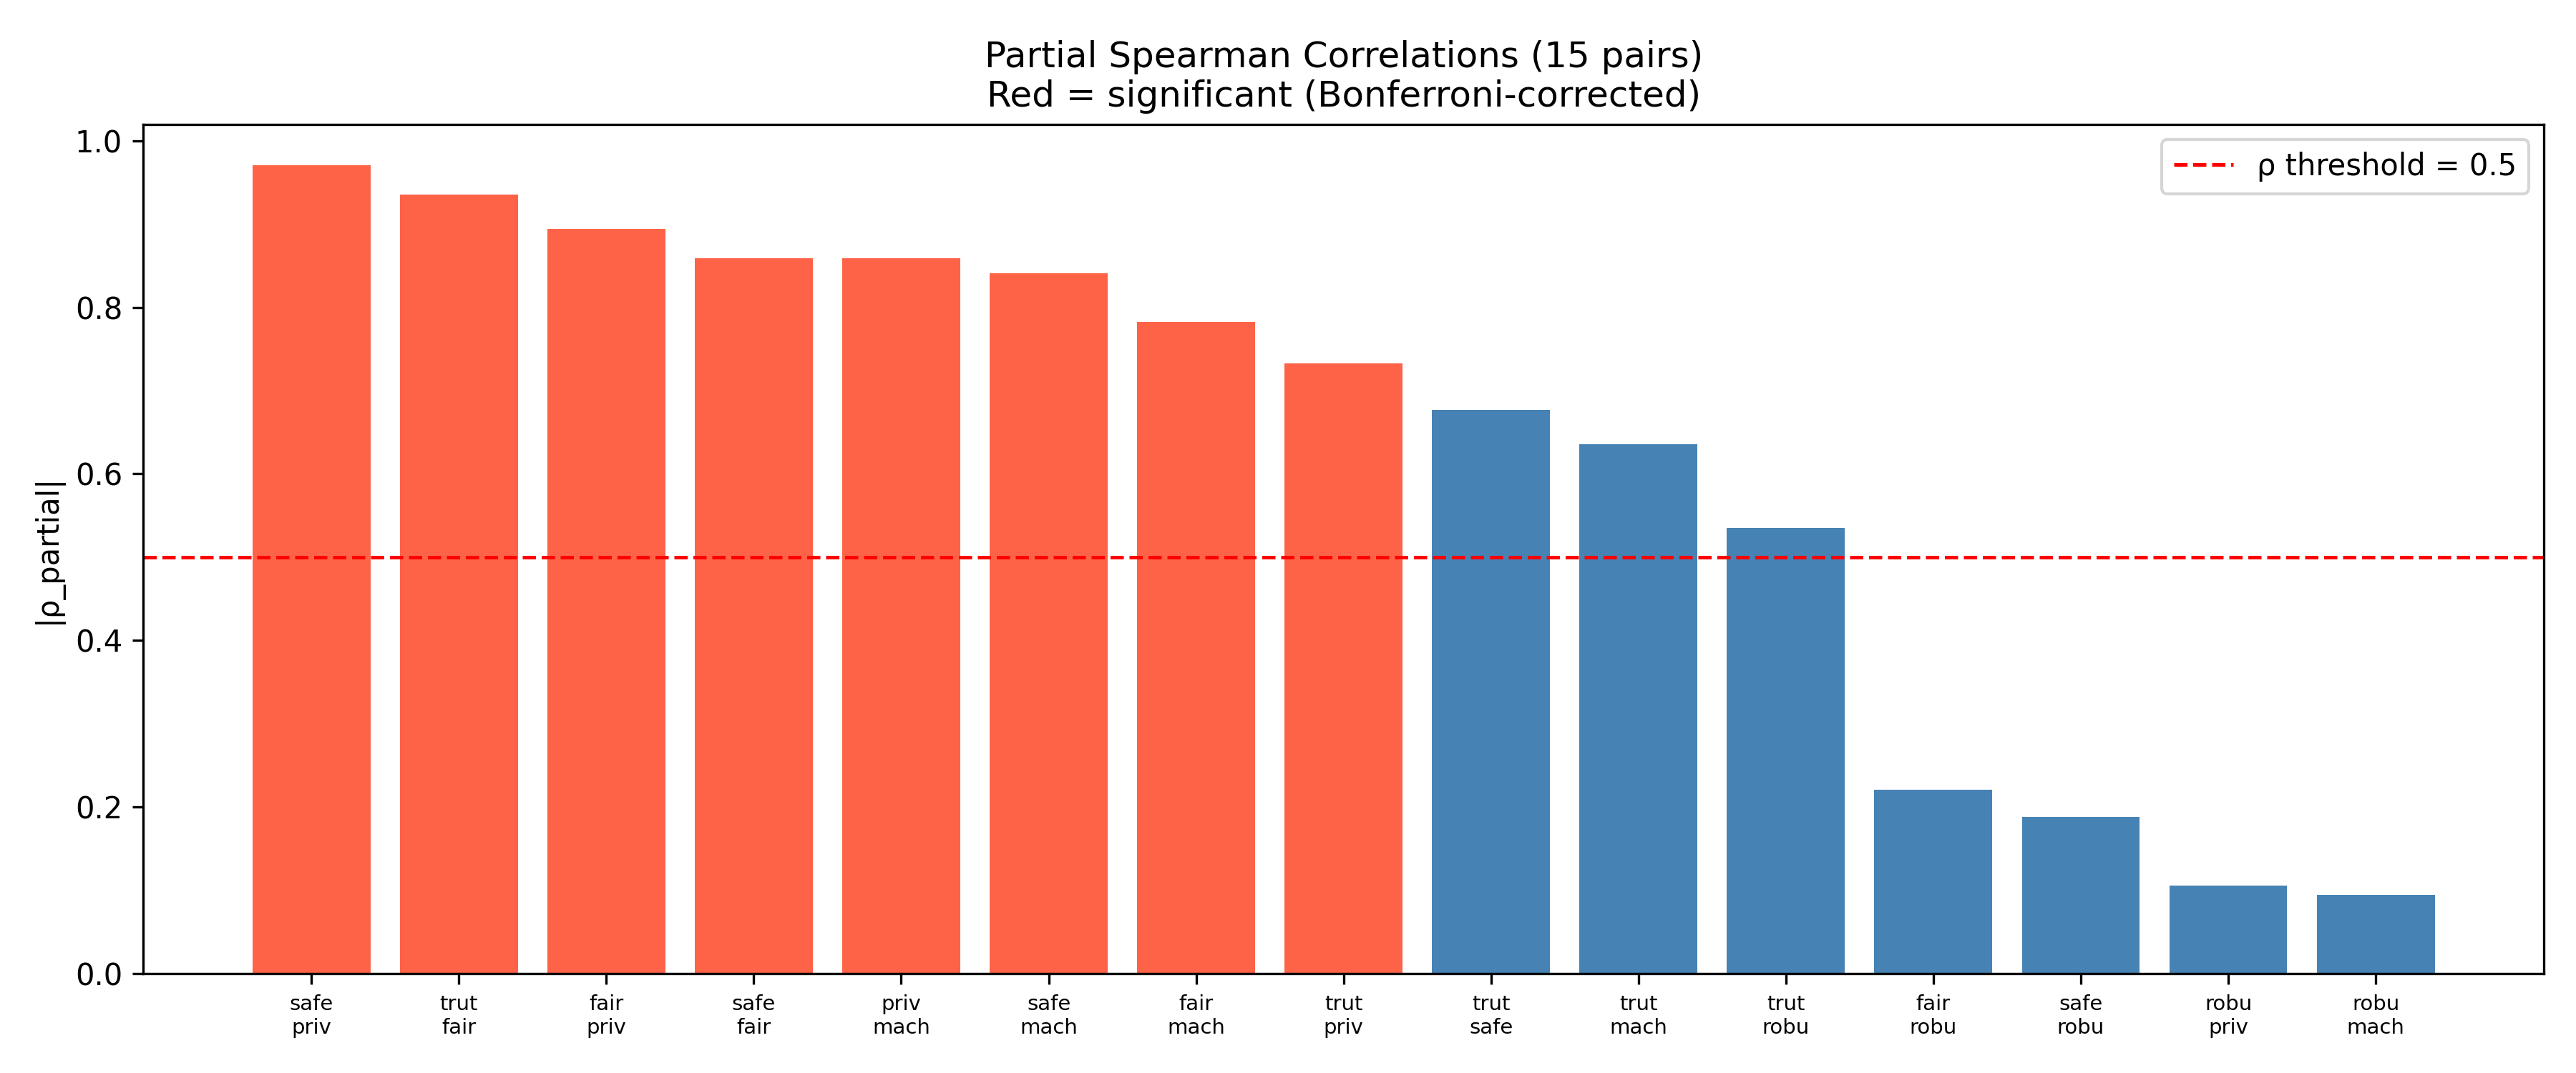
\includegraphics[width=\linewidth]{figures/01_bar.png}
\caption{Absolute partial Spearman correlation $|\rho_\text{partial}|$ for all 15 dimension pairs, sorted by magnitude. Red bars indicate Bonferroni-significant pairs ($p < 0.0033$). 8 of 15 pairs exceed the significance threshold.}
\label{fig:bar}
\end{figure}

\begin{figure}[h]
\centering
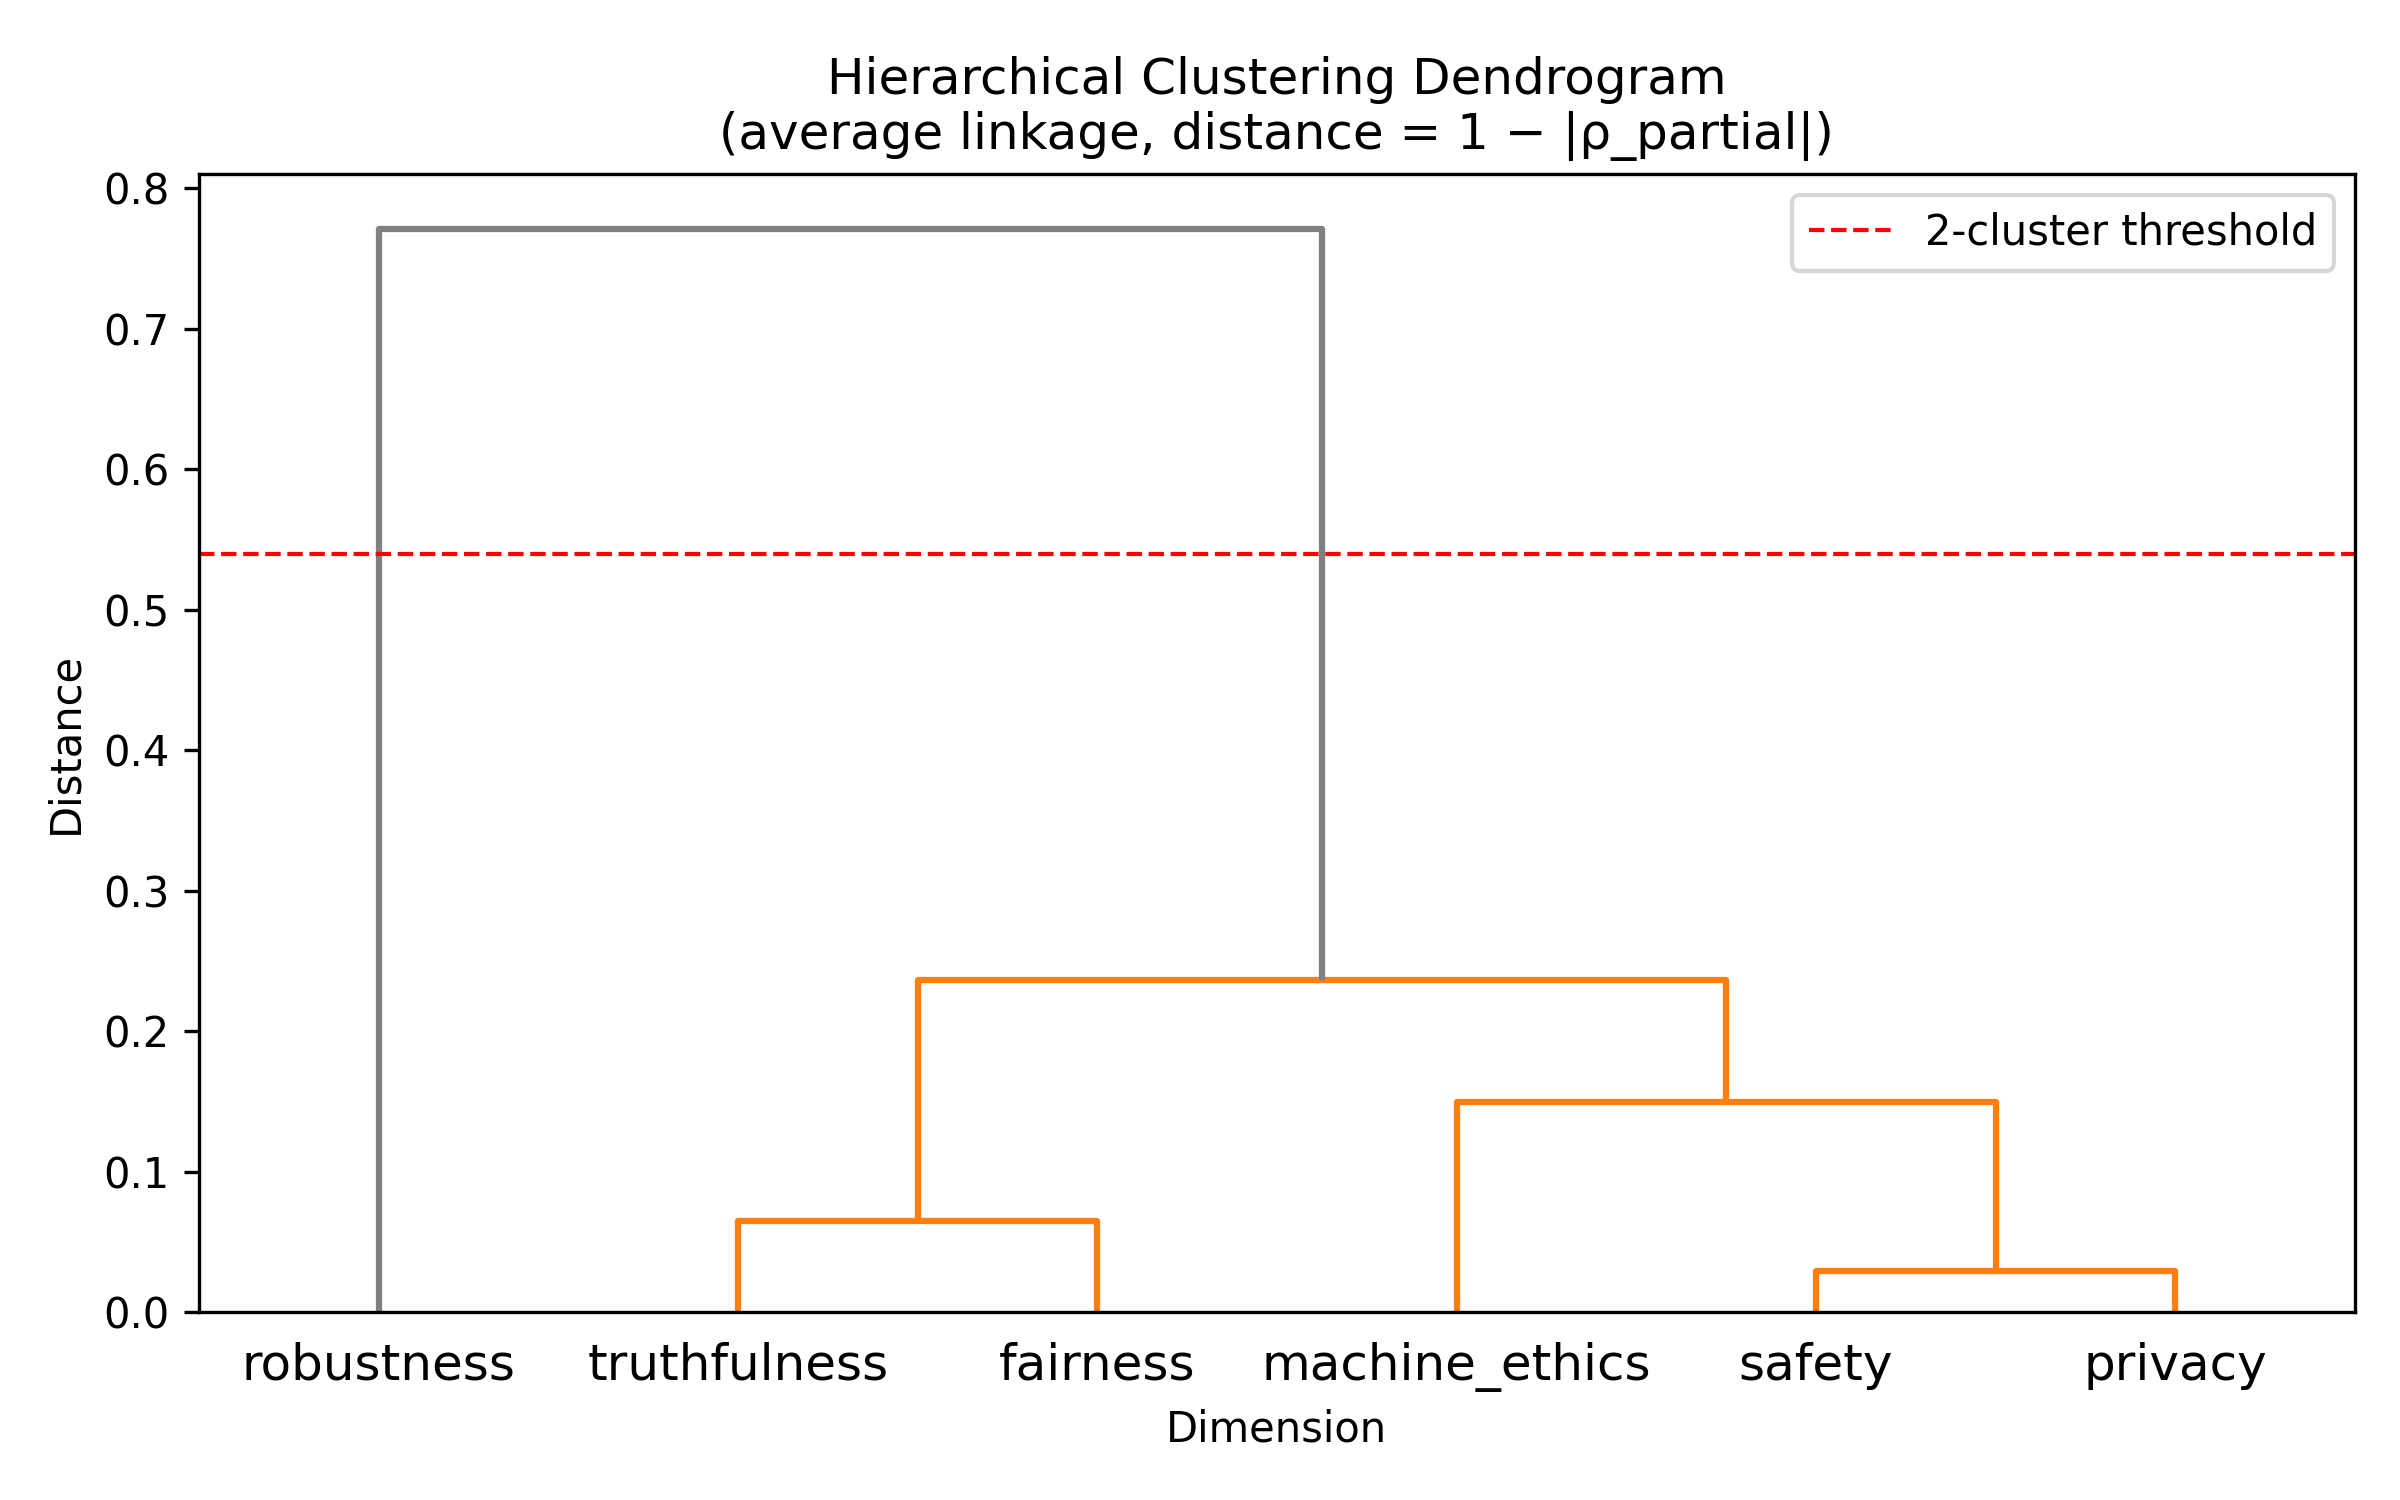
\includegraphics[width=0.8\linewidth]{figures/03_dendrogram.png}
\caption{Average-linkage hierarchical clustering dendrogram of the $6 \times 6$ partial Spearman distance matrix. The dashed line marks the 2-cluster cut: robustness branches early, confirming its isolation from the 5-dimension RLHF-shaped cluster.}
\label{fig:dendrogram}
\end{figure}

\begin{figure}[h]
\centering
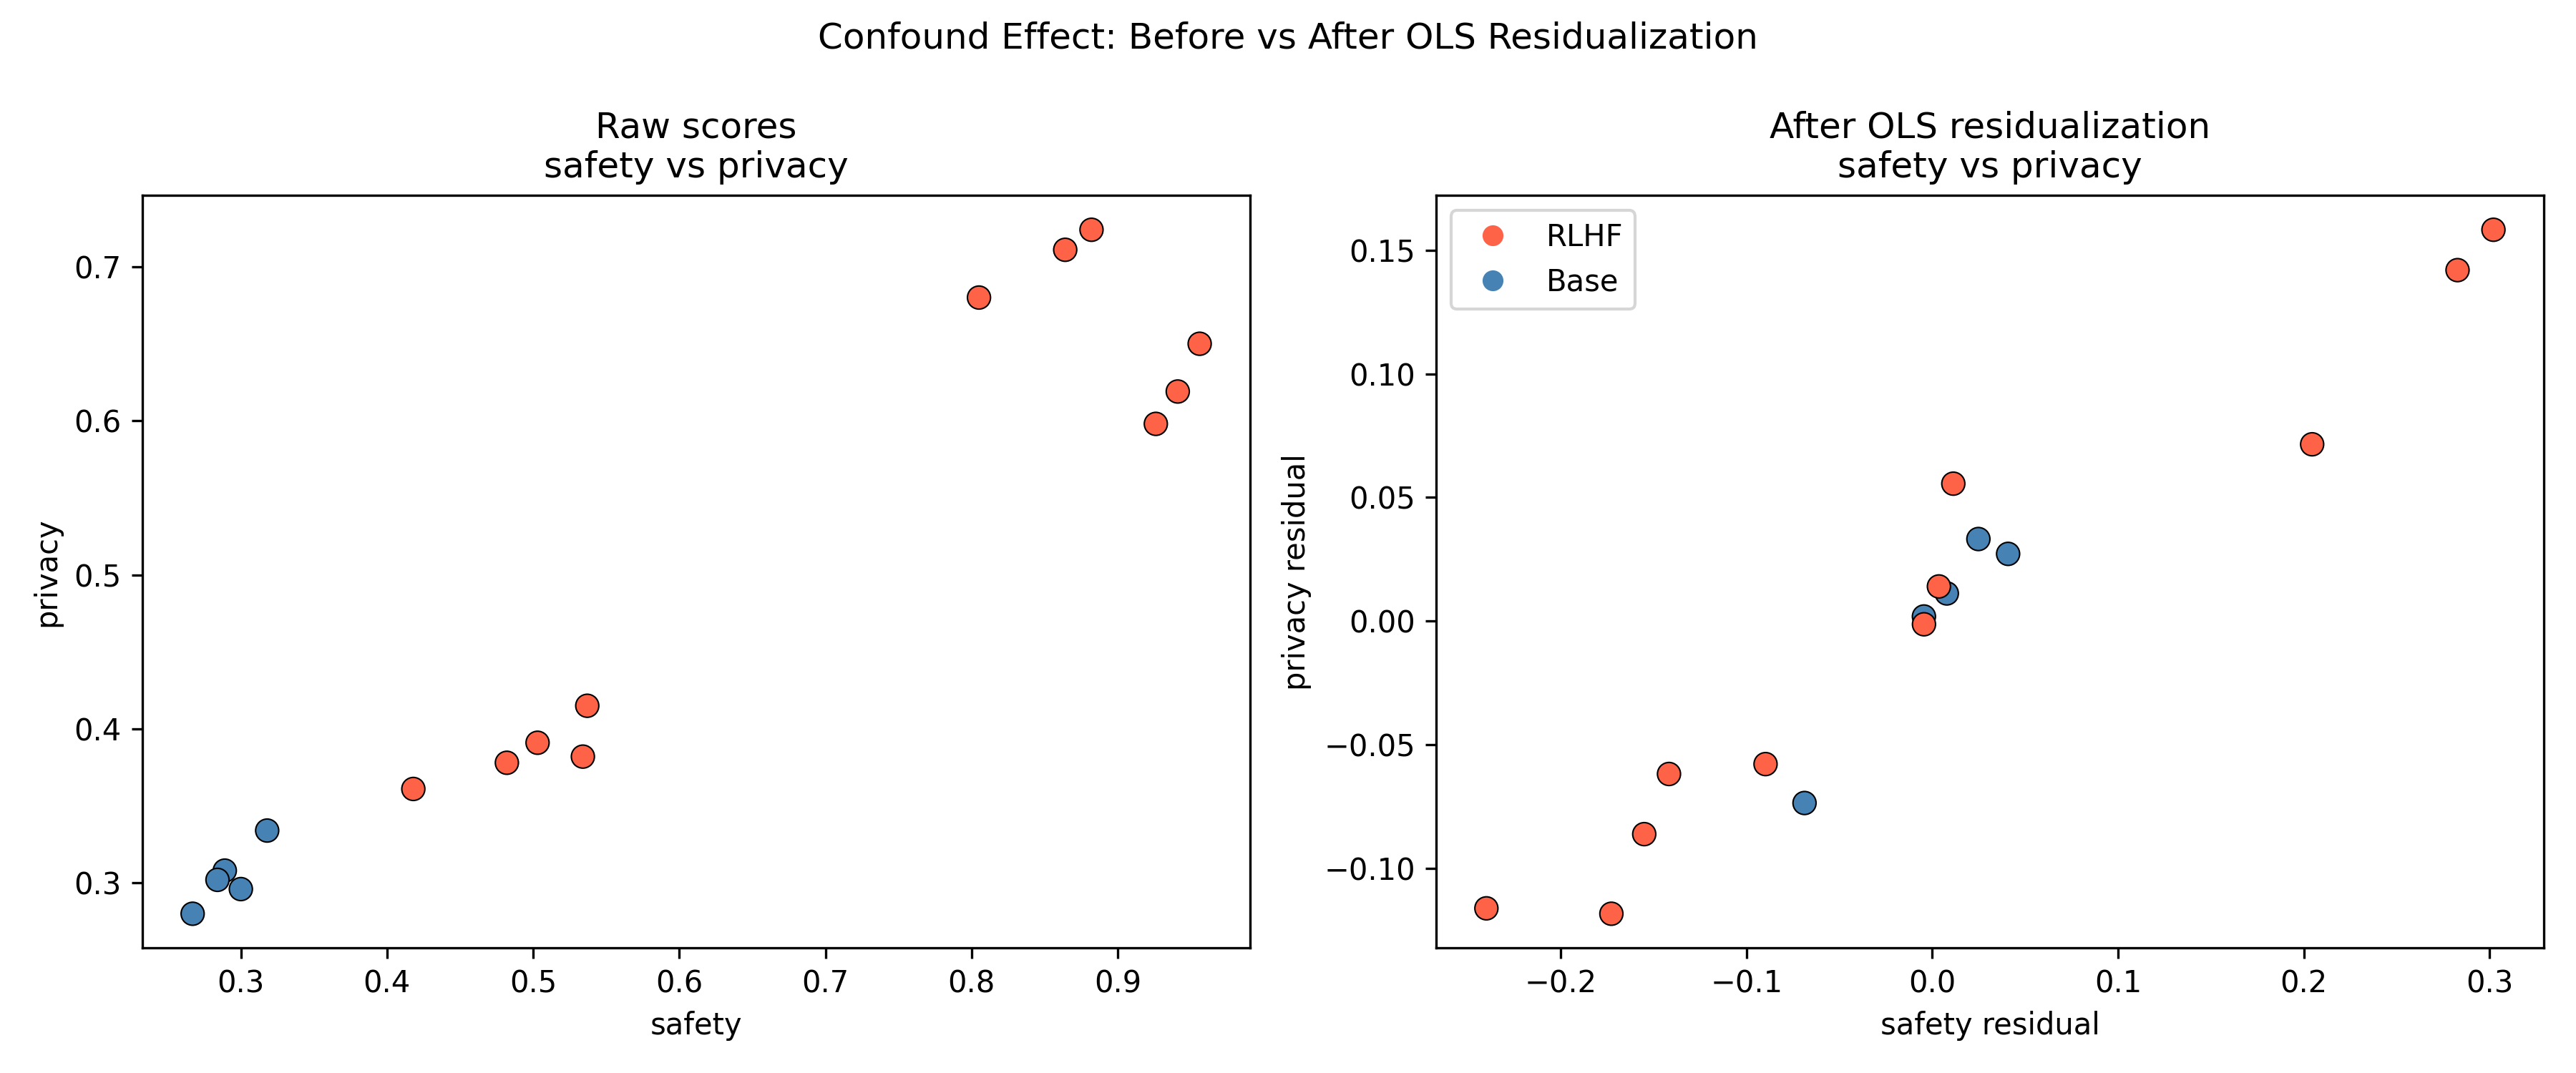
\includegraphics[width=0.8\linewidth]{figures/04_scatter.png}
\caption{OLS residualization demonstration for the safety--privacy pair ($\rho = 0.971$). Points colored by RLHF status show confound removal isolates the trustworthiness-specific correlation.}
\label{fig:scatter}
\end{figure}

\begin{figure}[h]
\centering
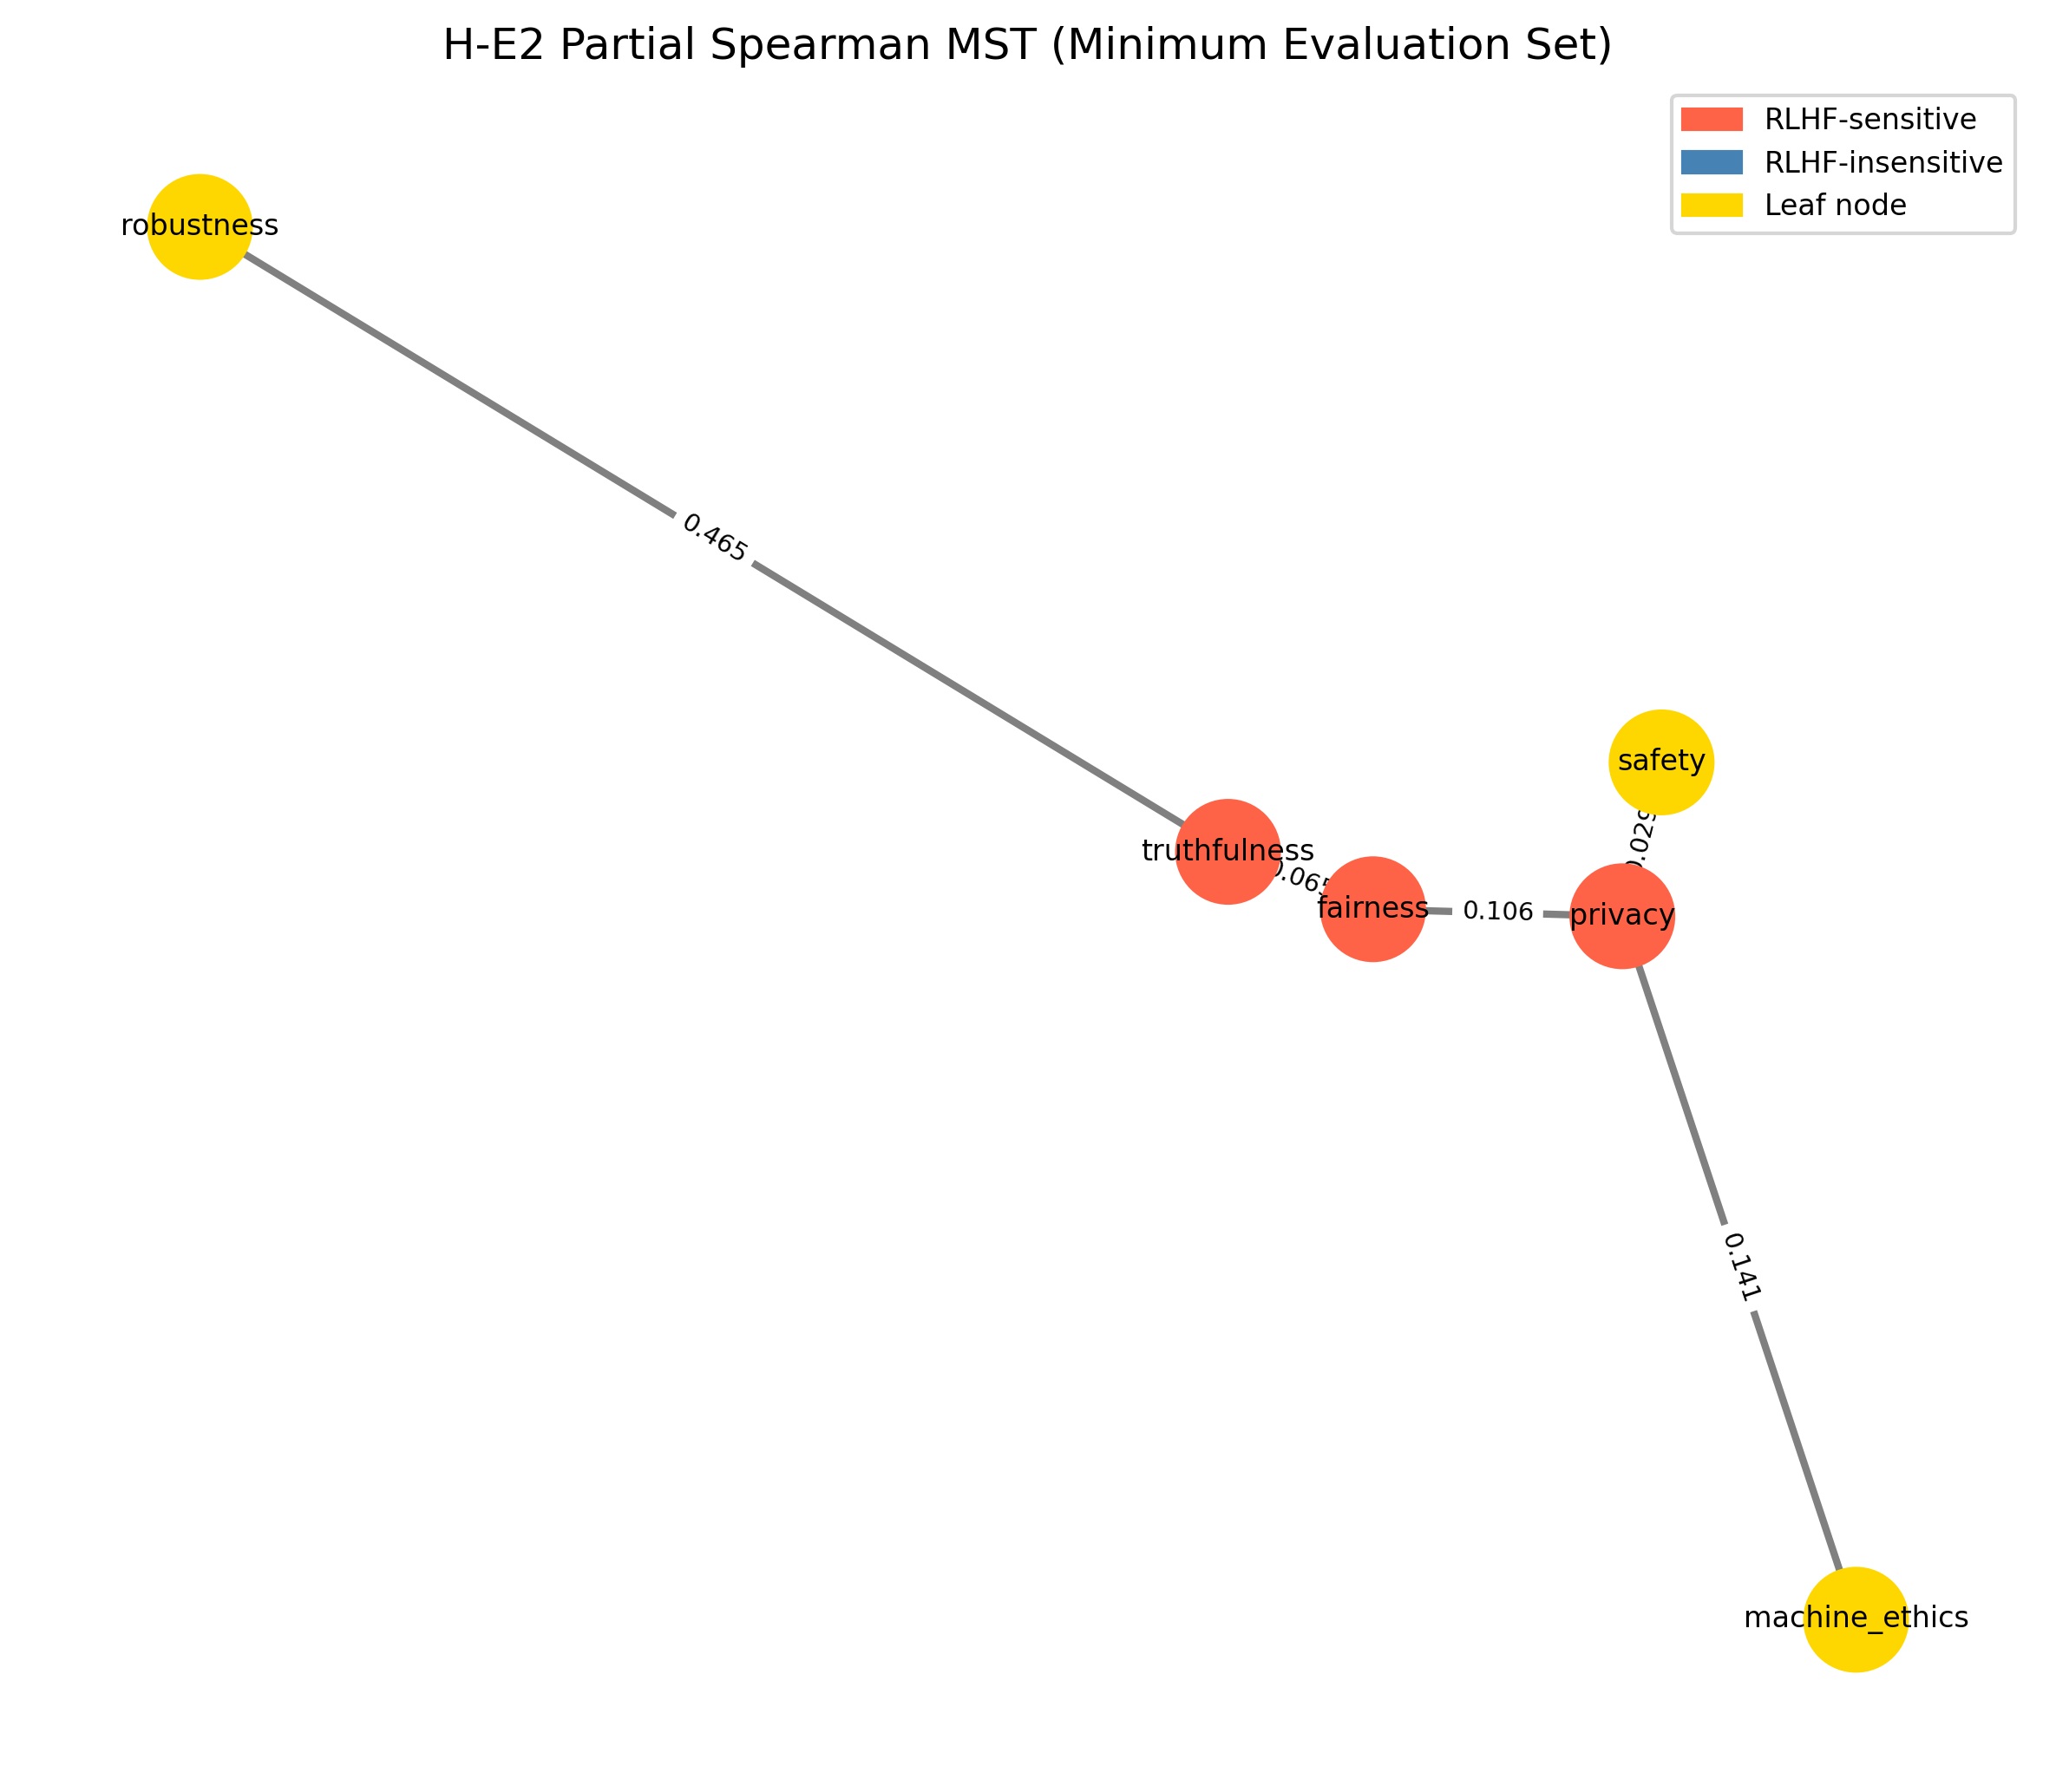
\includegraphics[width=0.7\linewidth]{figures/mst_graph.png}
\caption{Minimum spanning tree (MST) of the partial Spearman distance matrix. Hub nodes \{truthfulness, fairness, privacy\} form the 3-dimension minimum evaluation set. Leaf nodes (safety, robustness, machine\_ethics) are redundant for evaluation compression.}
\label{fig:mst}
\end{figure}

\begin{figure}[h]
\centering
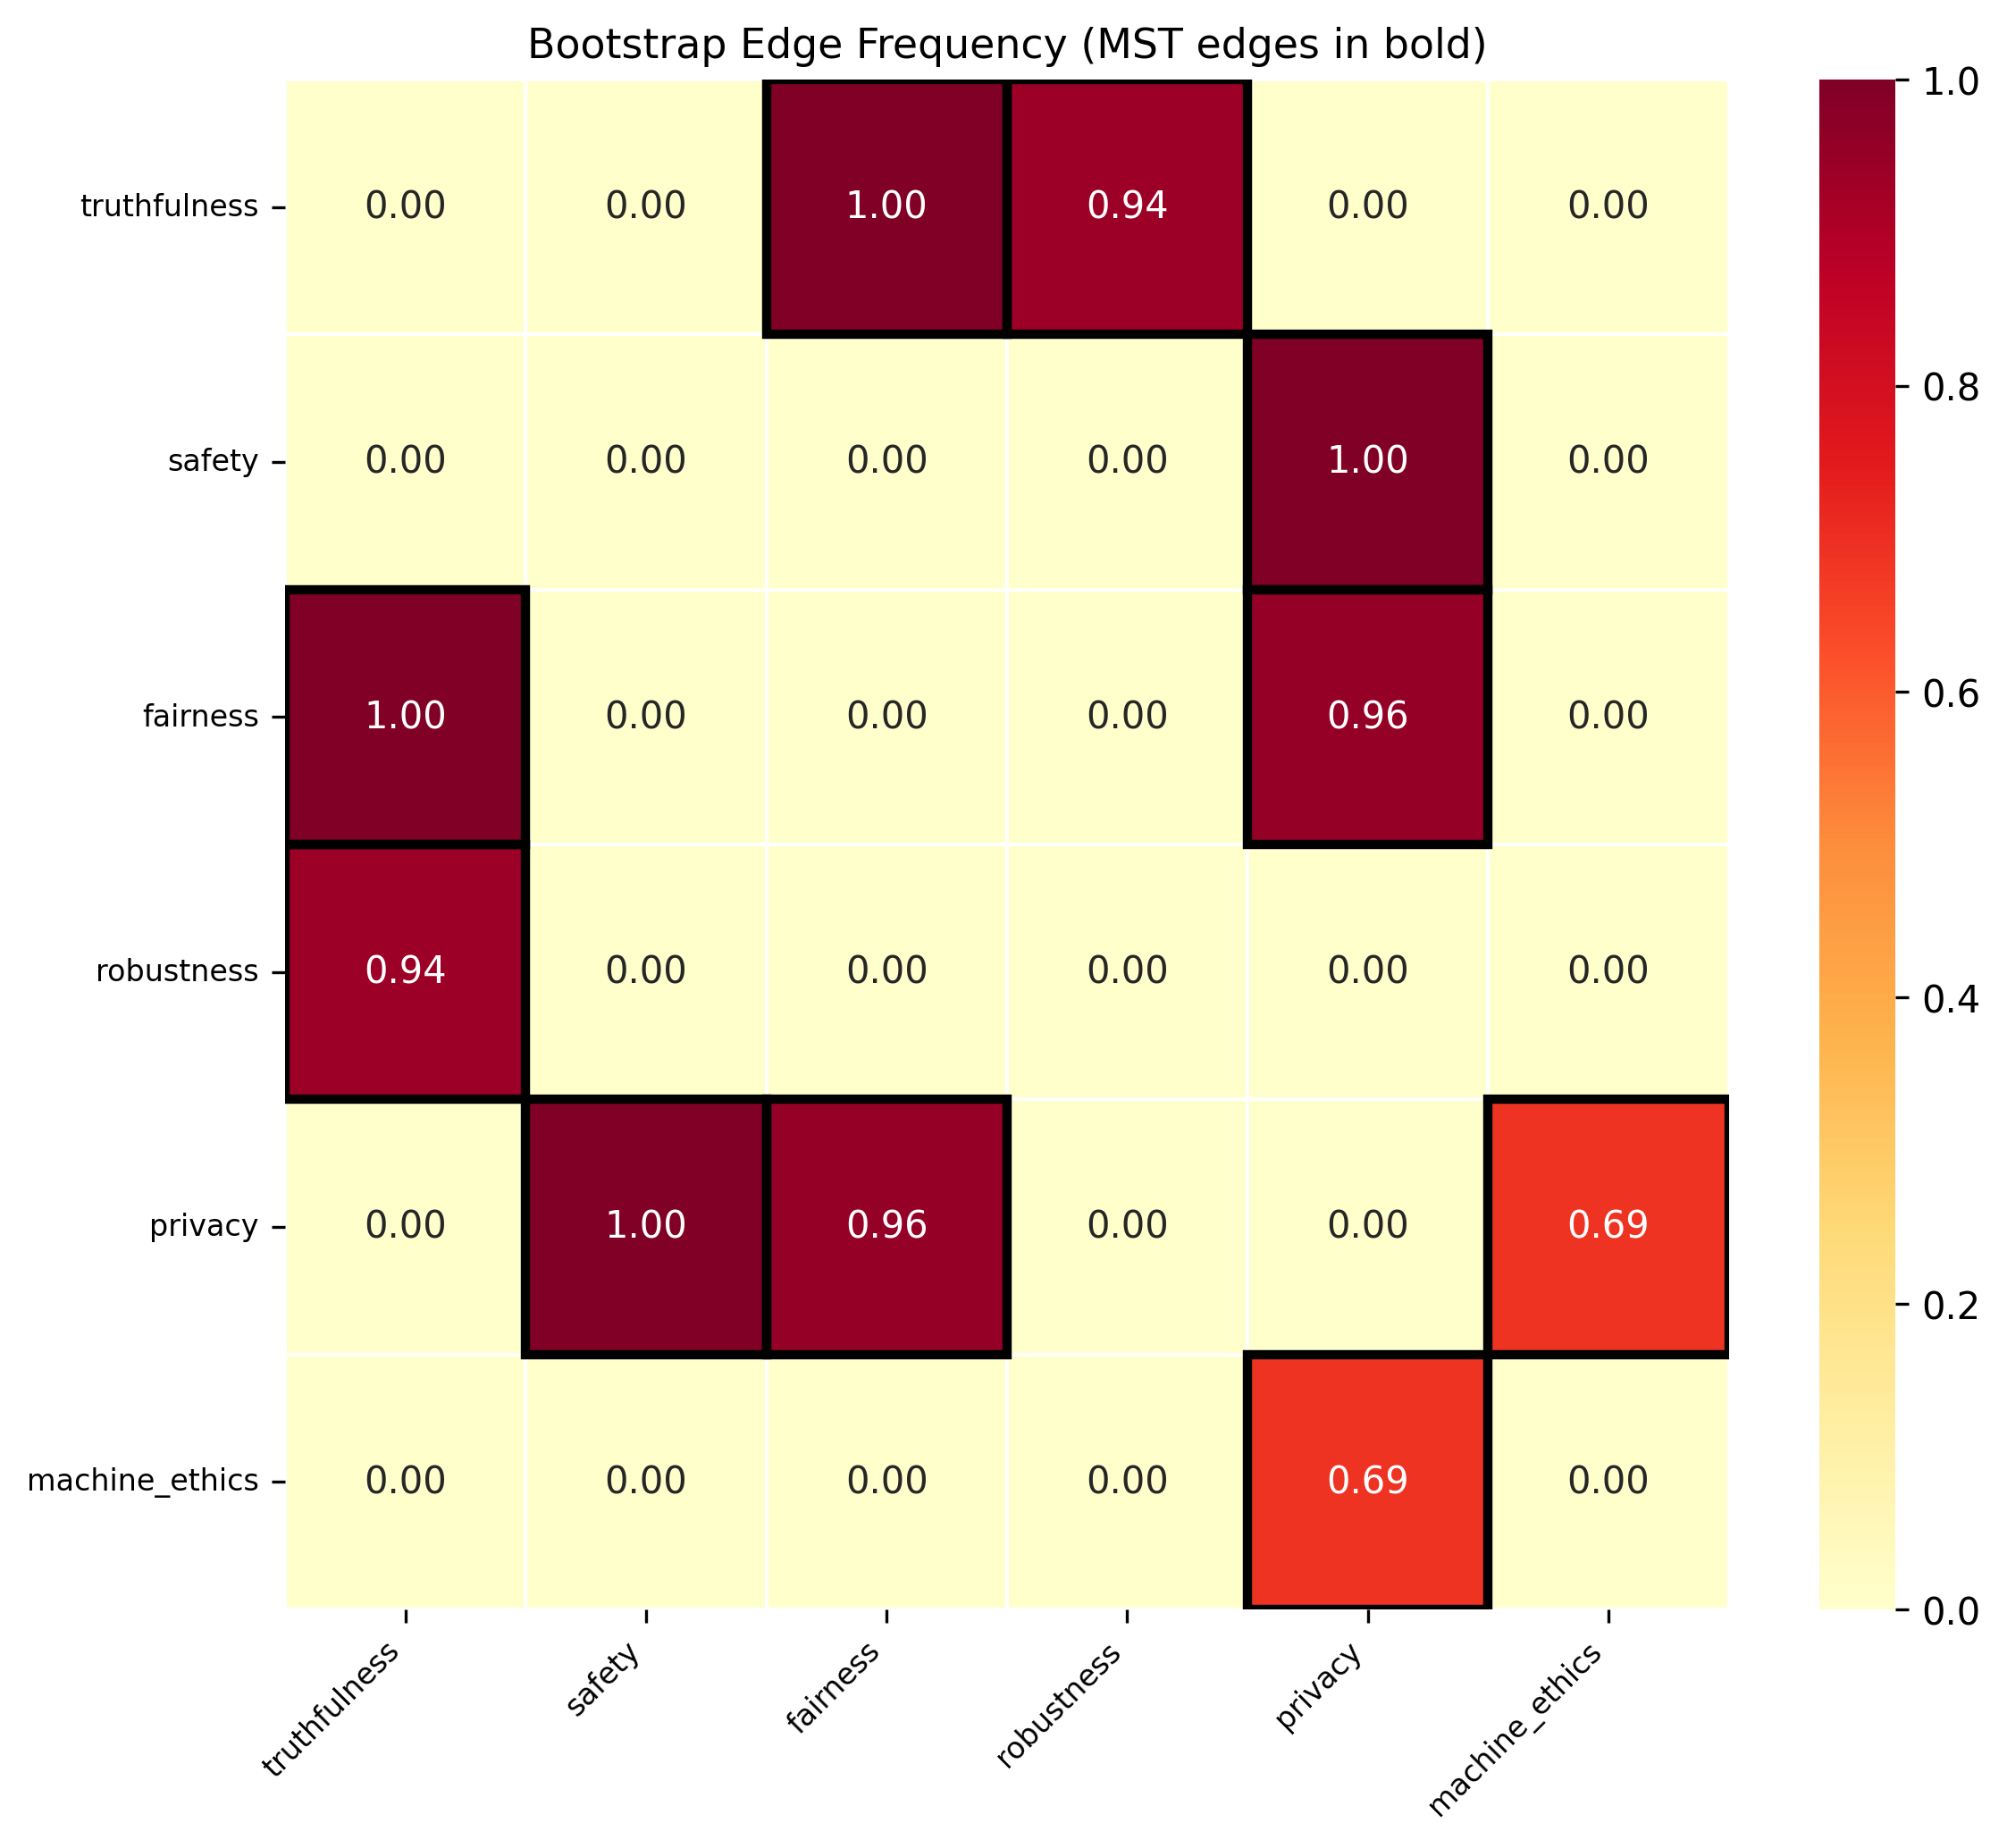
\includegraphics[width=0.8\linewidth]{figures/bootstrap_heatmap.png}
\caption{Per-edge bootstrap frequency heatmap (1000 resamples of 14/16 models). Four of five MST edges exceed 94\% stability. The machine\_ethics--privacy edge at 68.8\% reflects near-tie geometry at $n=16$.}
\label{fig:bootstrap}
\end{figure}

\begin{figure}[h]
\centering
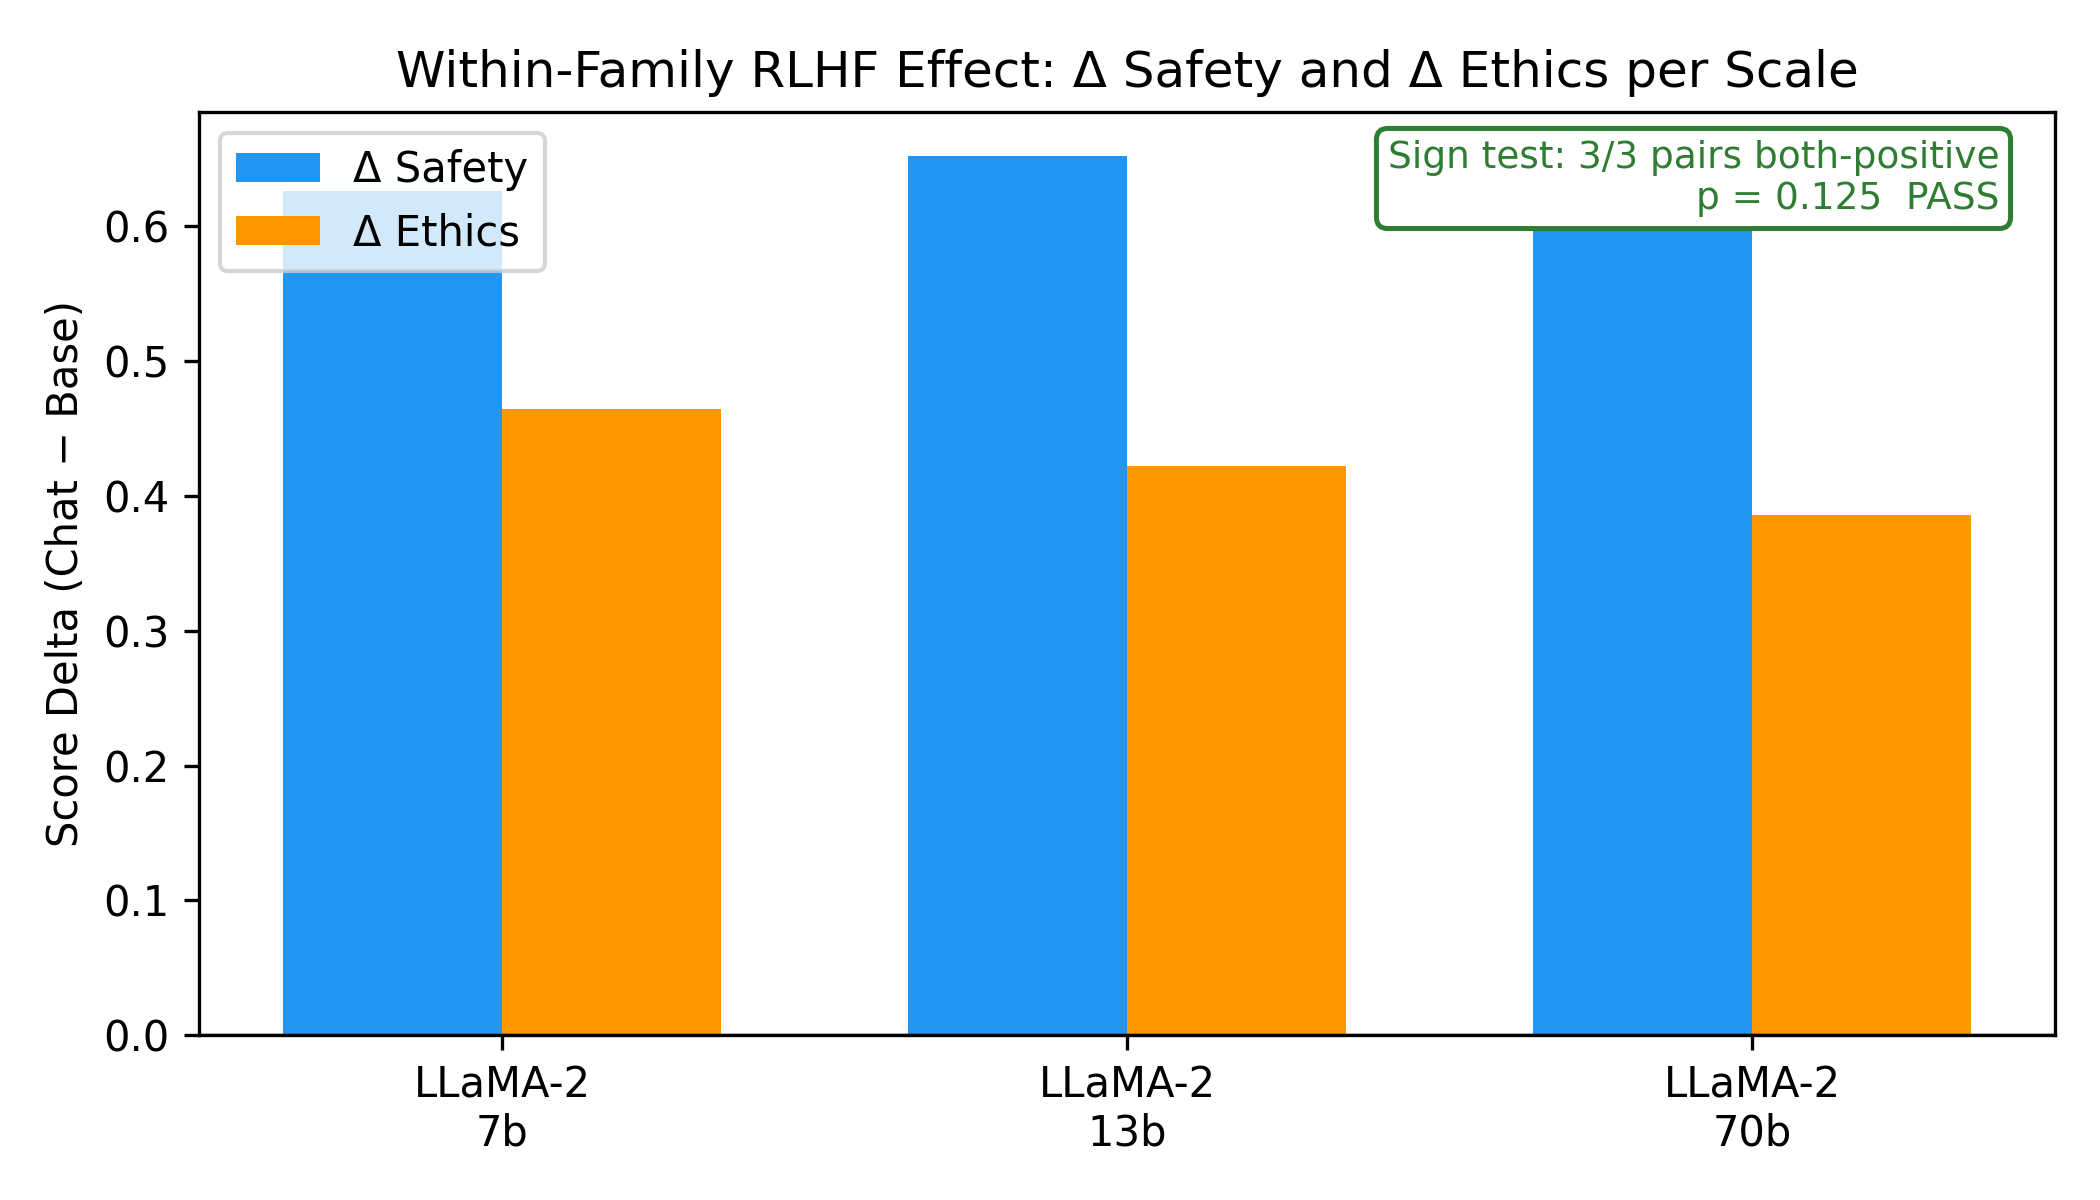
\includegraphics[width=0.8\linewidth]{figures/fig2_within_family_deltas.png}
\caption{RLHF-induced score changes ($\Delta = \text{Chat} - \text{Base}$) for safety and machine\_ethics across LLaMA-2 7B, 13B, and 70B. All six bars are positive, demonstrating joint optimization at every scale.}
\label{fig:deltas}
\end{figure}

\begin{figure}[h]
\centering
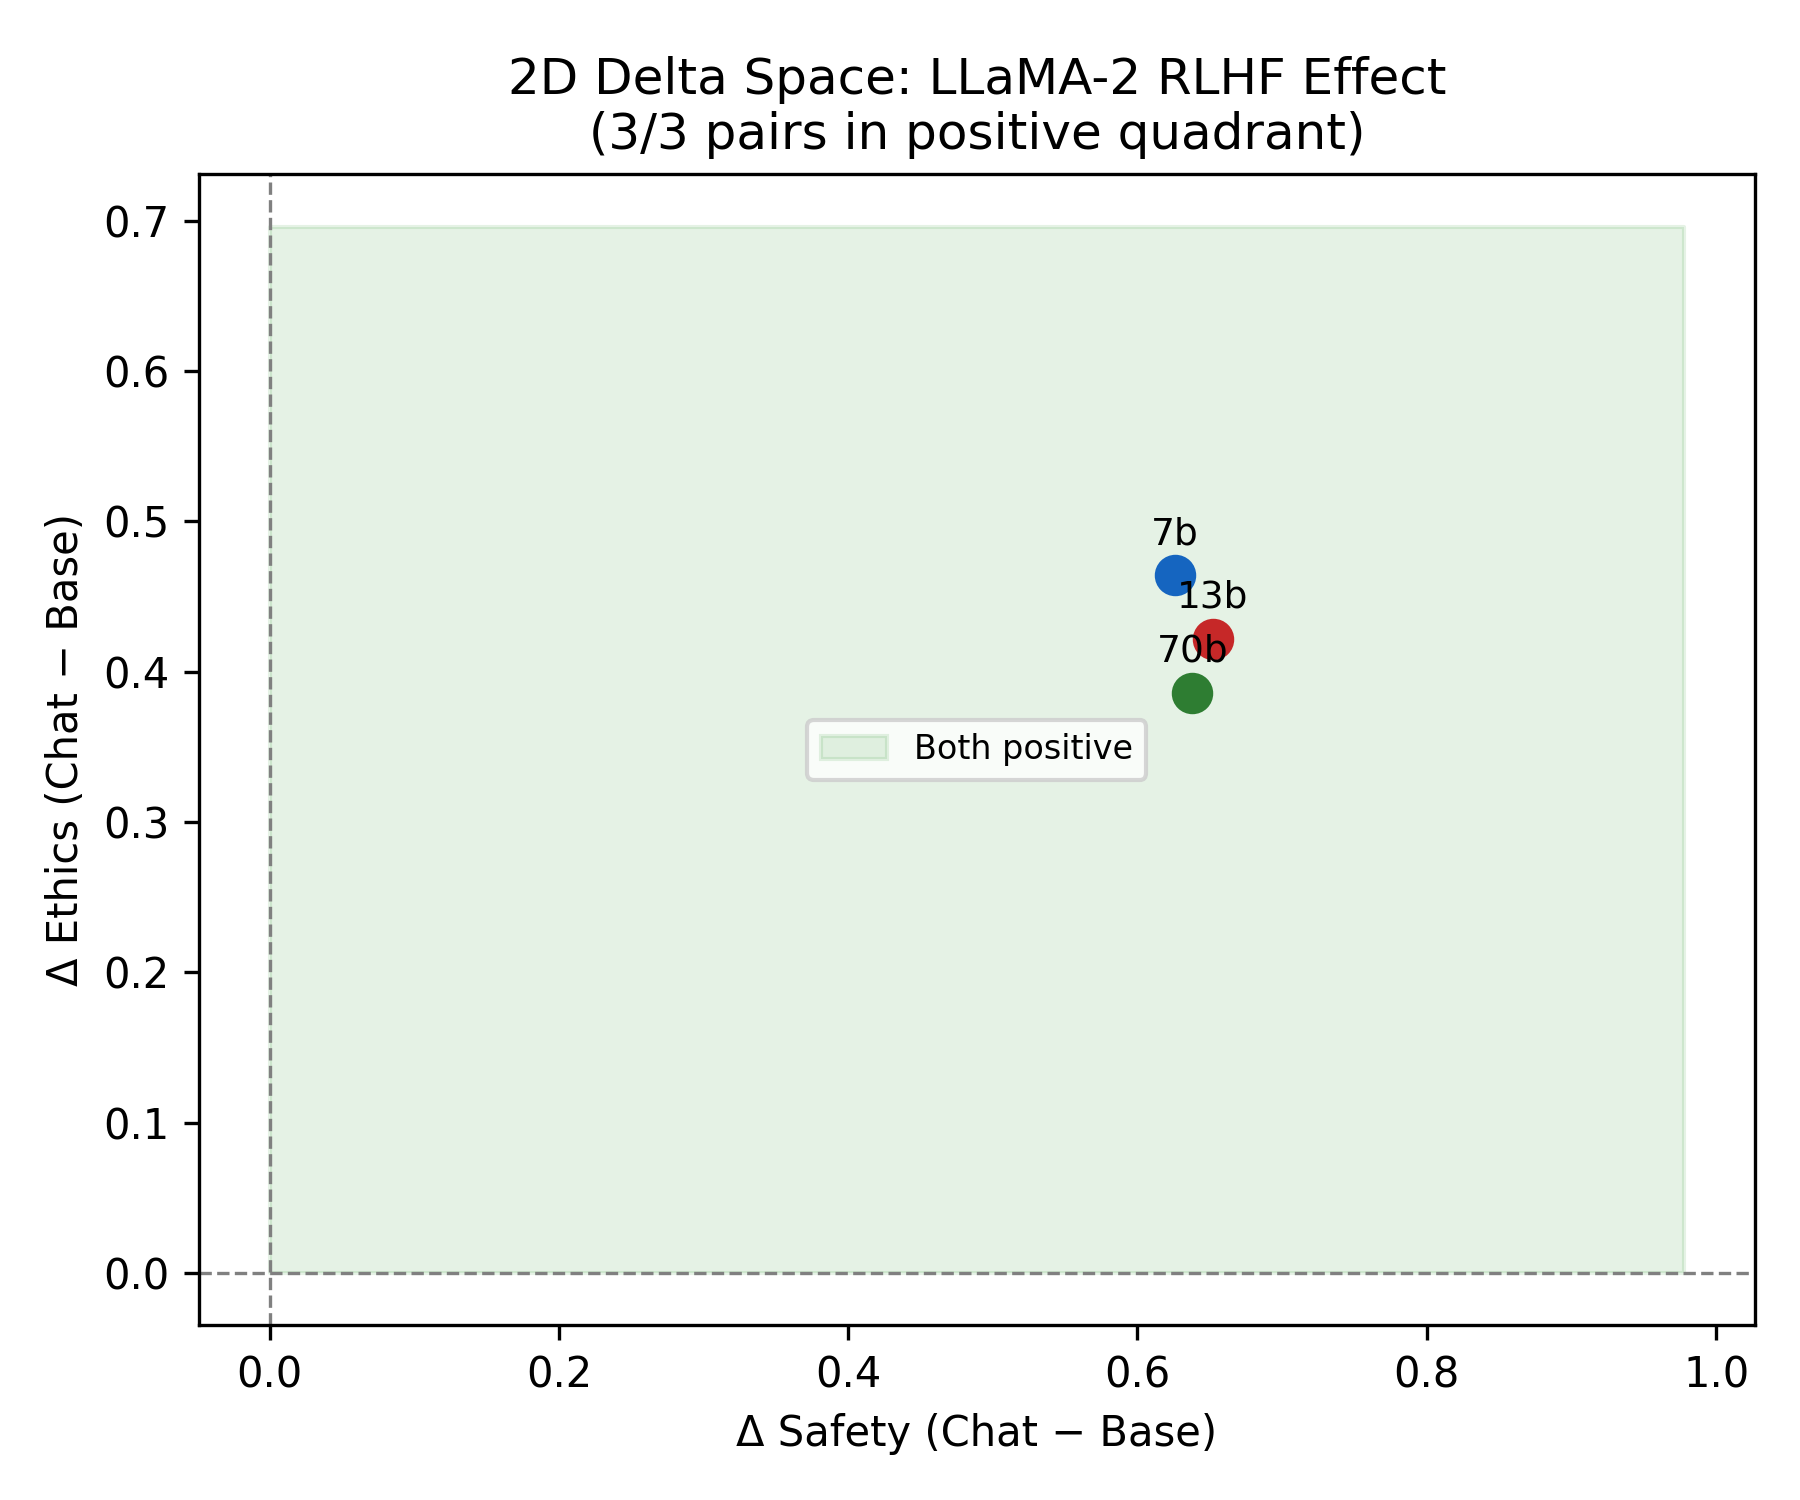
\includegraphics[width=0.7\linewidth]{figures/fig4_delta_2d.png}
\caption{2D delta space scatter ($\Delta_\text{safety}$ vs.\ $\Delta_\text{ethics}$) for LLaMA-2 within-family pairs. All three scale points land in the upper-right quadrant (both positive), confirming joint RLHF optimization.}
\label{fig:delta2d}
\end{figure}

\begin{figure}[h]
\centering
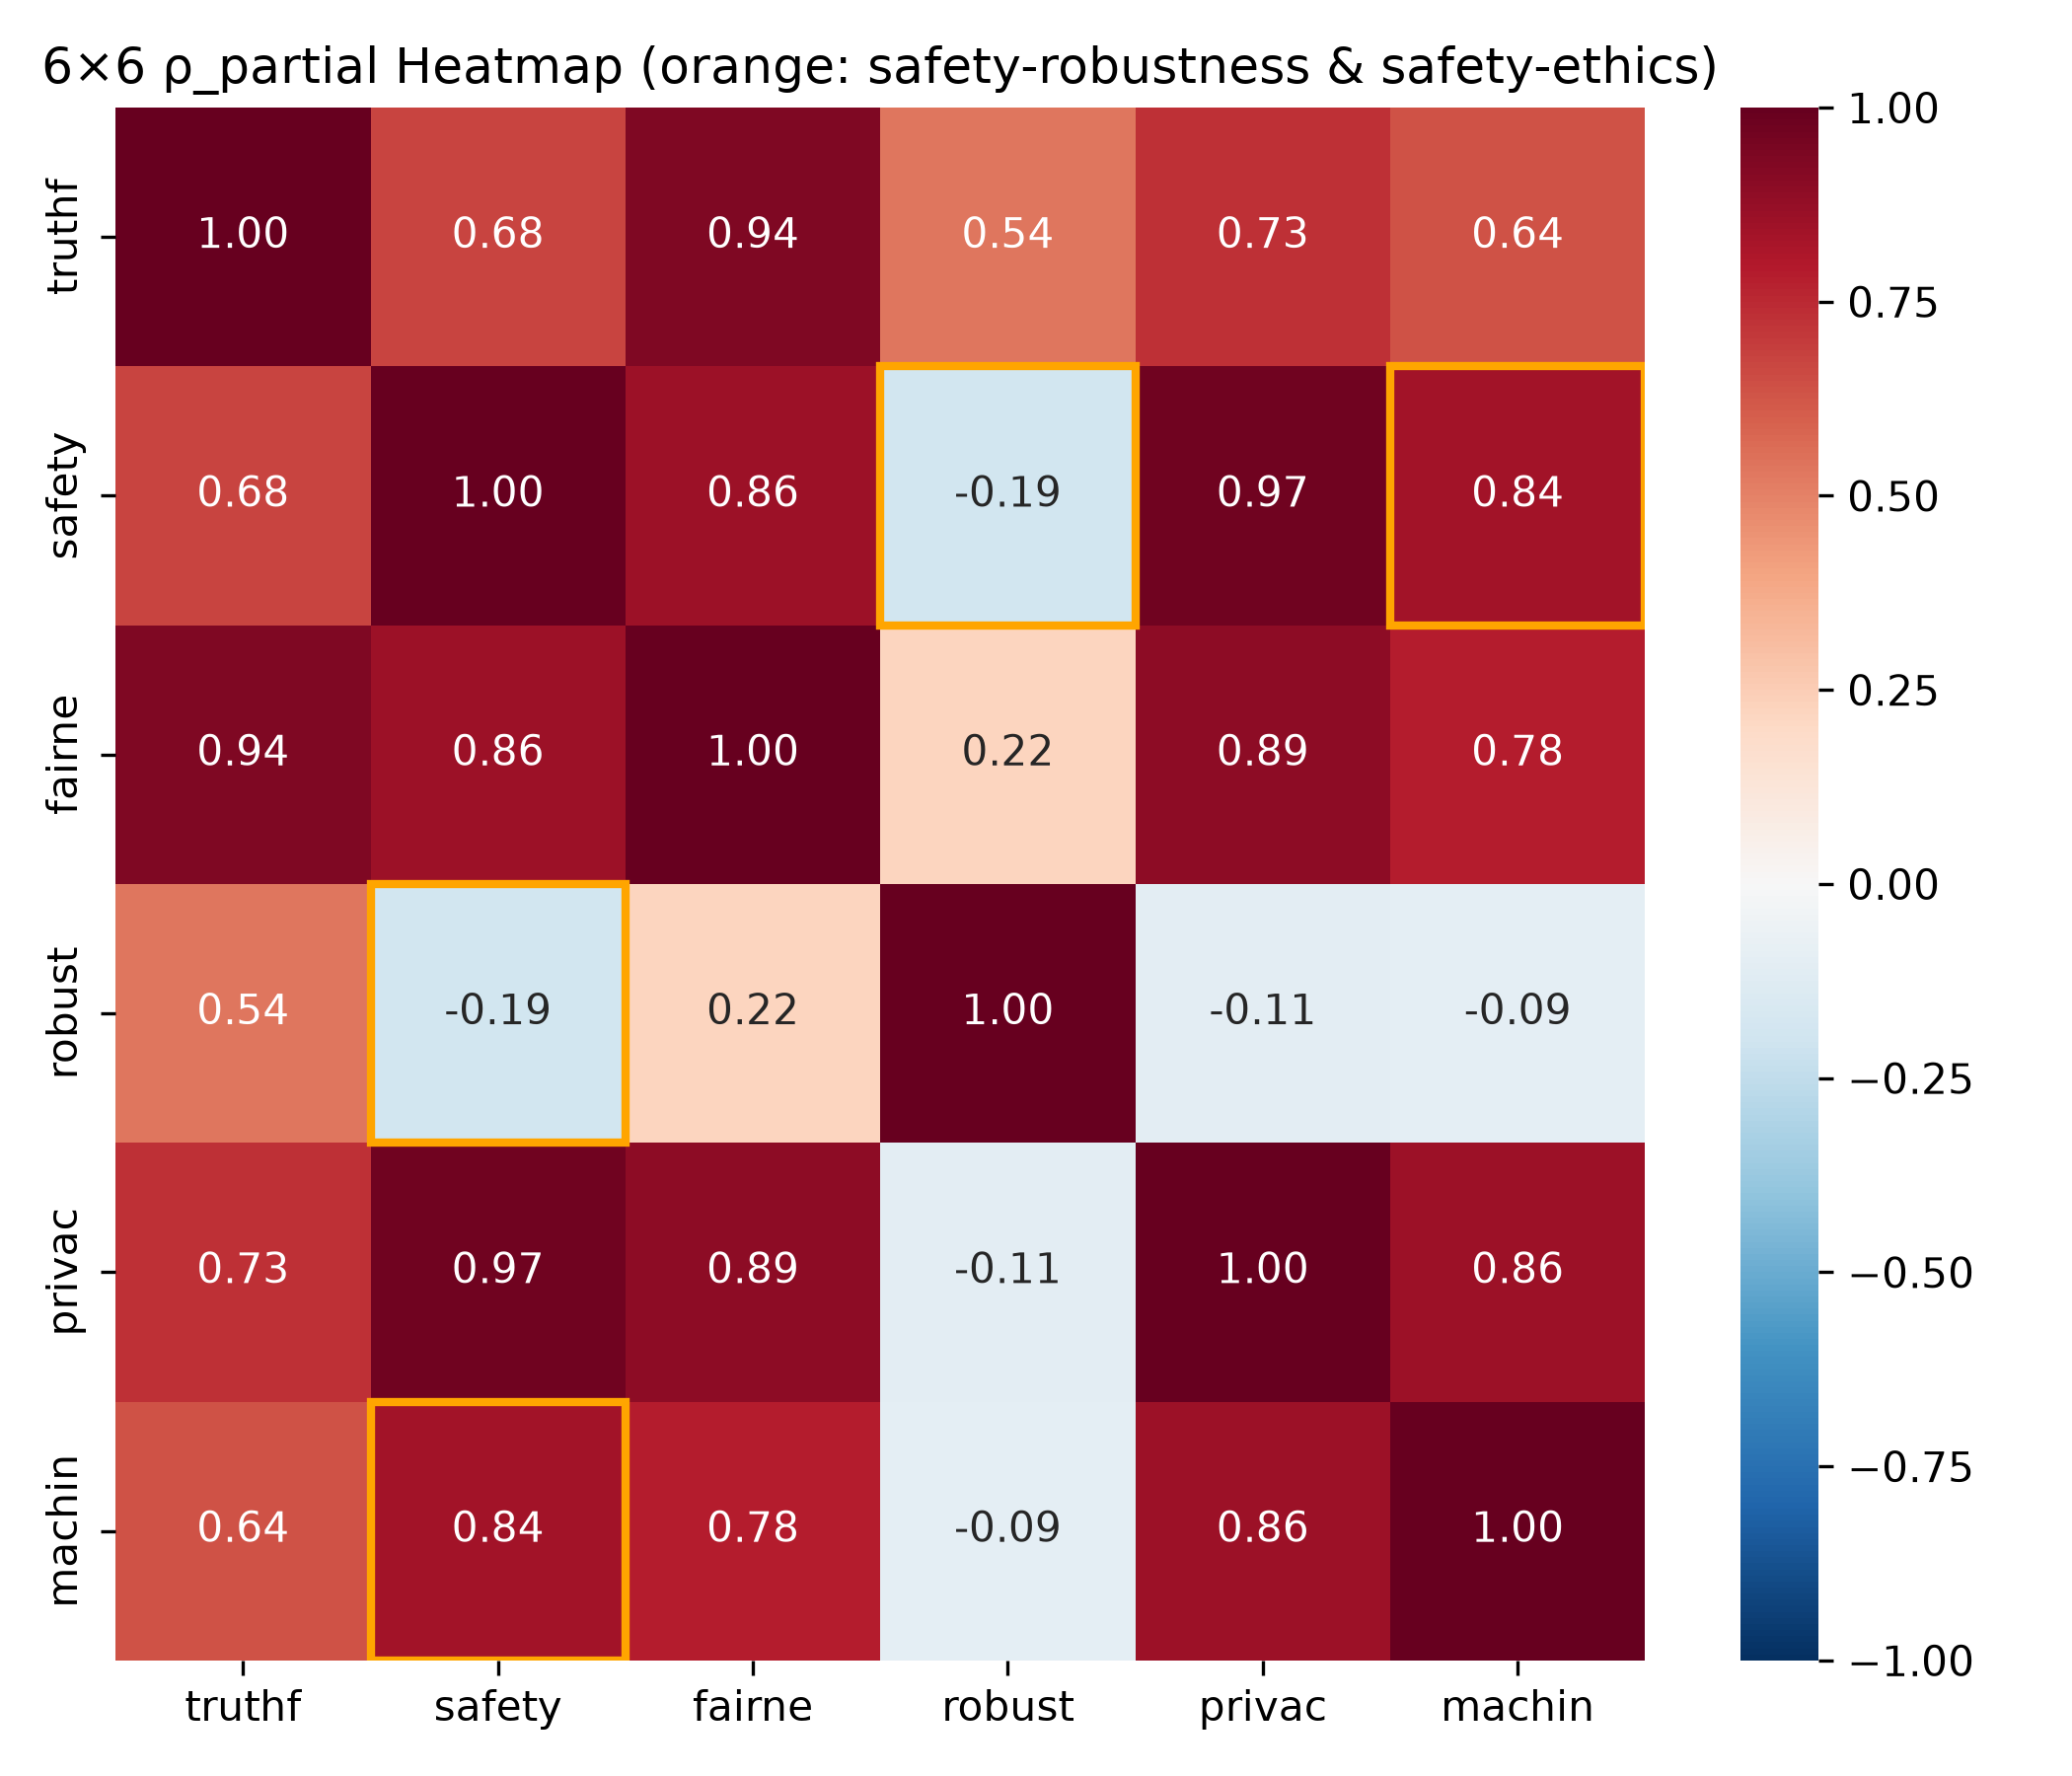
\includegraphics[width=0.8\linewidth]{figures/rho_heatmap_h_m2.png}
\caption{Full $6 \times 6$ partial Spearman correlation heatmap with the safety--robustness cell highlighted. The directional negative value ($\rho = -0.188$) is consistent with a safety-robustness tension but does not reach Bonferroni significance at $n=16$.}
\label{fig:rho_highlight}
\end{figure}

\begin{figure}[h]
\centering
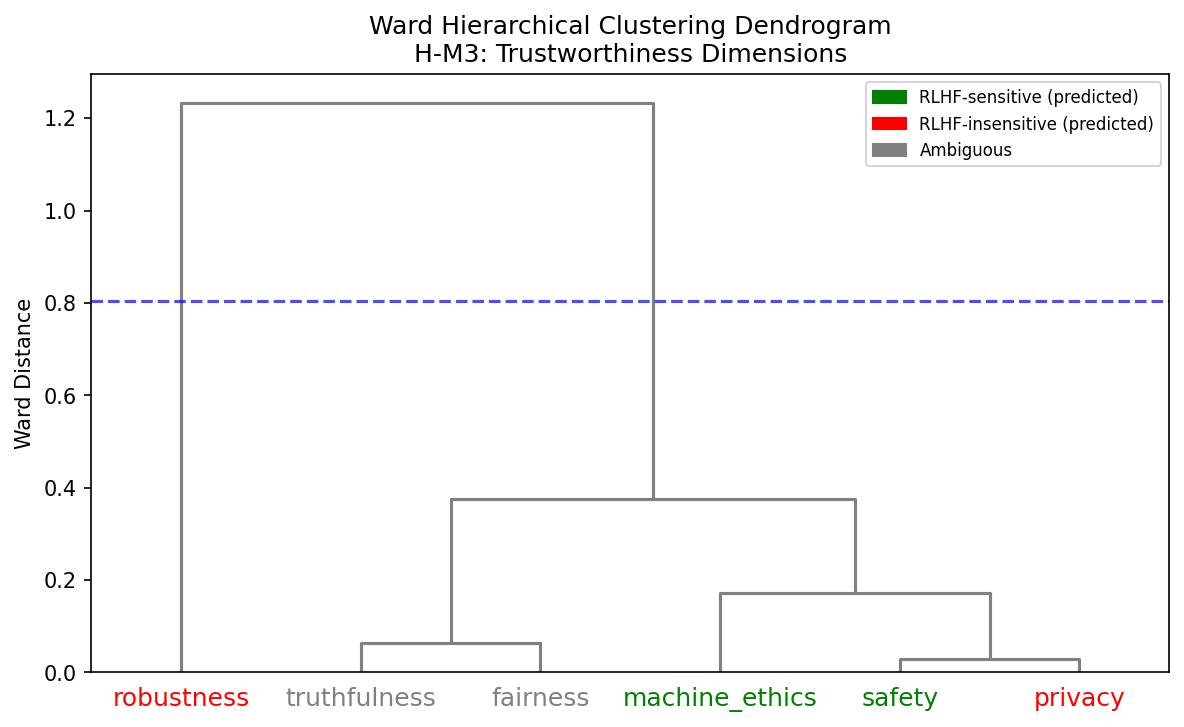
\includegraphics[width=0.8\linewidth]{figures/dendrogram_ward.png}
\caption{Ward-linkage dendrogram confirming the 2-cluster structure (silhouette = 0.637). The functional split is \{robustness\} vs.\ \{all other 5 dimensions\}.}
\label{fig:dendrogram_ward}
\end{figure}

\begin{figure}[h]
\centering
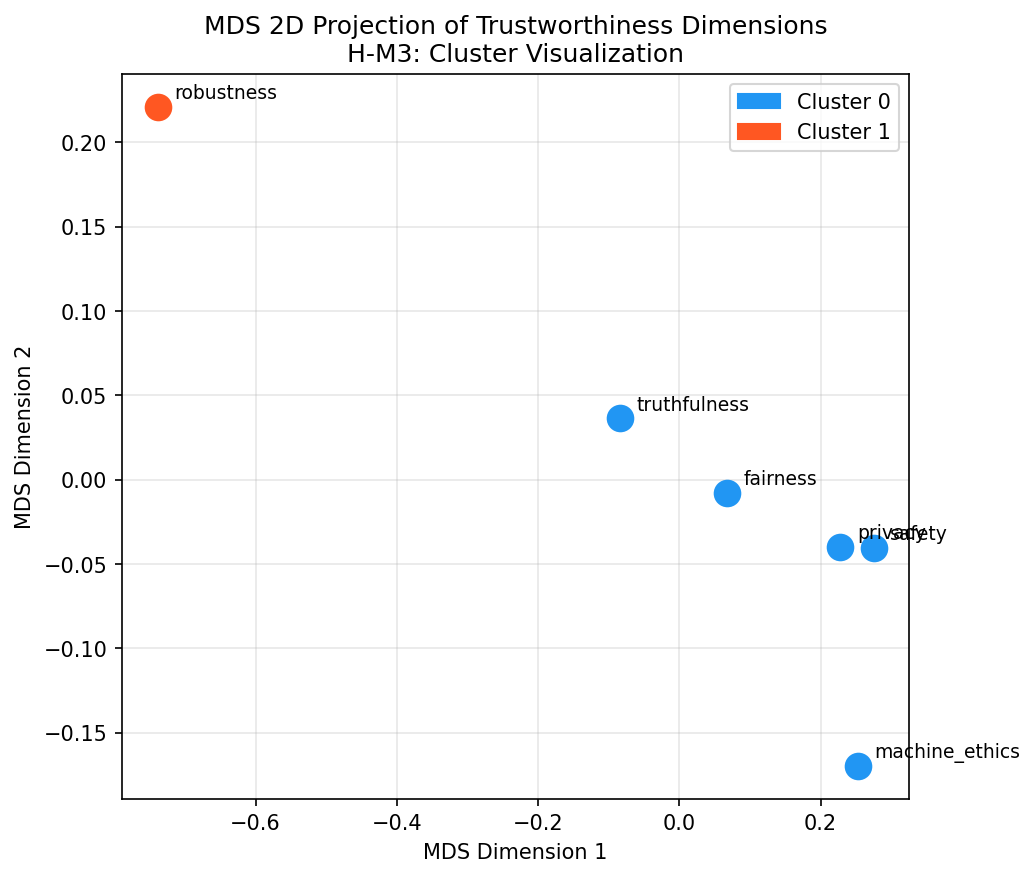
\includegraphics[width=0.8\linewidth]{figures/mds_projection.png}
\caption{2D multidimensional scaling (MDS) projection of the $6 \times 6$ partial Spearman distance matrix. Robustness is geometrically separated from the tight 5-dimension cluster.}
\label{fig:mds}
\end{figure}

\begin{figure}[h]
\centering
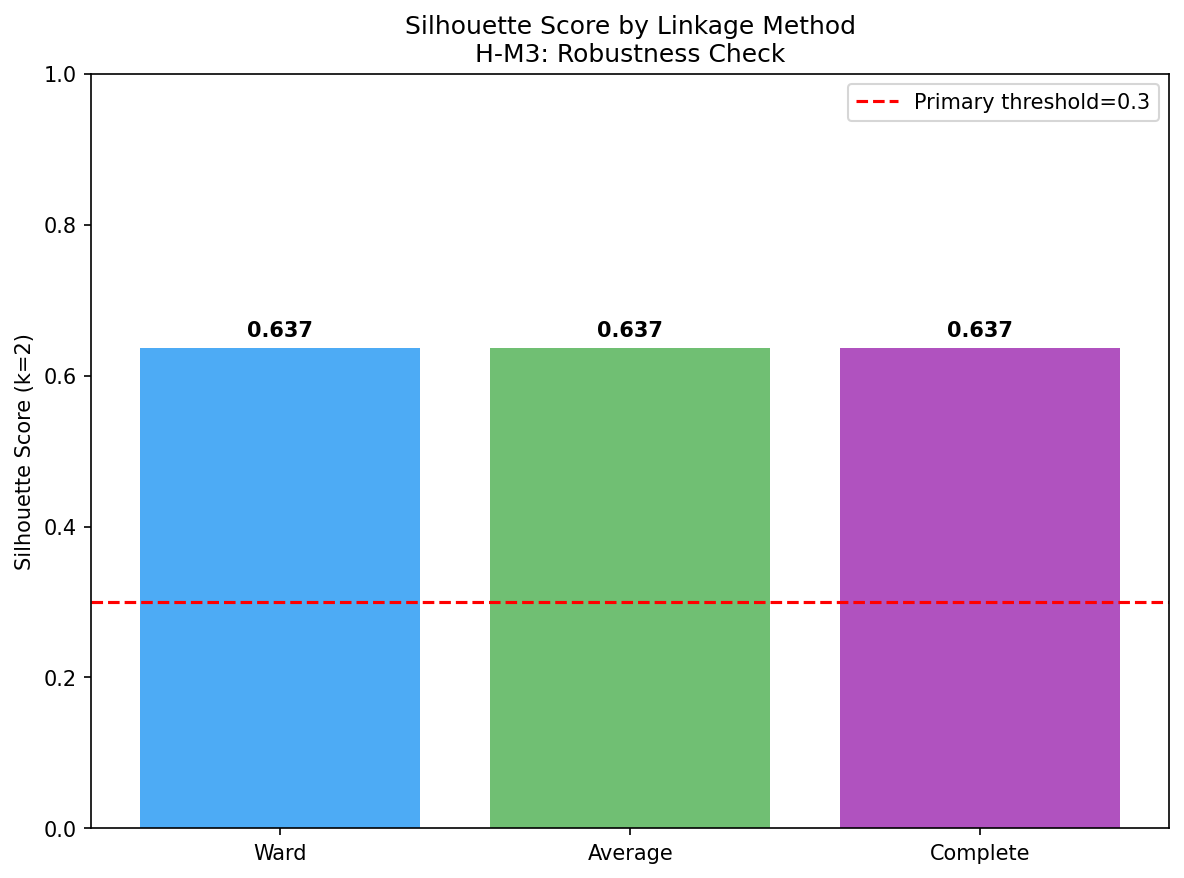
\includegraphics[width=0.8\linewidth]{figures/silhouette_comparison.png}
\caption{Silhouette scores for $k=2$ clustering using Ward, average, and complete linkage methods (all = 0.637) vs.\ $k=3$ (0.500). Identical scores across linkage methods confirm the 2-cluster structure is not a methodological artifact.}
\label{fig:silhouette}
\end{figure}
